\documentclass{beamer}
\usepackage[latin1, utf8]{inputenc}
\usepackage{wrapfig}
\usepackage{framed}

\useoutertheme[height=0pt,left]{sidebar}
\usecolortheme{seahorse}
\setbeamercolor*{titlelike}{parent=structure}
\useinnertheme{circles}
\setbeamertemplate{frametitle}[default][right]

\title{Les robots ressemblant à l'humain sont-ils vraiment utiles ?}
\author{Christian LASSERRE\\ Théophile GUILBAUD}
\institute{ENSEIRB-MATMECA}
\date{}

\begin{document}
\begin{frame}
  \titlepage
\end{frame}

\begin{frame}
  \tableofcontents
\end{frame}

\section{Ressemblance}
\begin{frame}
  RESSEMBLANCE
\end{frame}

\subsection{Le(s) Géminoide(s)}
\begin{frame}{Histoire}
  Professeur
\end{frame}

\begin{frame}{Auteur}
\end{frame}

\subsection{Caractéristiques}
\begin{frame}{Geminoide HI-4}
  \begin{framed}
    \begin{wrapfigure}{l}{40mm}
      \centering
      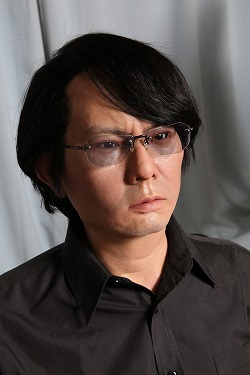
\includegraphics[width=40mm]{data/HI-4}
      \caption{Geminoïde HI-4}
    \end{wrapfigure}
    Il était une fois ...
  \end{framed}
\end{frame}

\begin{frame}{Geminoide HI-2}
\end{frame}

\begin{frame}{Geminoide F}
  (il y a aussi le DK...)
  convention social -> uniquement physique
\end{frame}

\subsection{Conclusion}
\begin{frame}{ça ressemble à un humain}
\end{frame}

\section{L'intéraction}
\begin{frame}
  INTERACTION
\end{frame}

\subsection{Télénoïde}
\begin{frame}{Présentation}
  Caractéristiques et évolution
  imiter l'humain sans but spécifique...
\end{frame}

\subsection{Utilité}
\begin{frame}
  possibilité d'utilisation :
  accueil hotel/aéroport
  peut être un sex symbol mais c'est tout (Rq : utilité de Nabilla)
\end{frame}

\begin{frame}{Avenir}
  aider l'homme
  ..
\end{frame}

\subsection{Conclusion}
\begin{frame}
  Robot Inhabituel, contre exemple de ce qu'on attend d'un robot.
  Aucune étude de proxémie, convention sociale développée, etc...
\end{frame}

\end{document}
